%   /*
%       Author : Subramanya J <subramanyajaradhya@gmail.com>
%   */

%   /* Definitions */
%   /* Modify these as needed */
\def \collegename {B. M. S. College Of Engineering}

\def \course {CRYPTOGRAPHY}
\def \coursecode {(23CS4ESCRP)}
\def \projectname {ChaCha20}

\def \one {Sarthaka Mitra GB (1BM23CS305)}
\def \two {Shaikh Uzair Ahmed (1BM23CS307)}
\def \three {Shashank U  (1BM23CS314)}
\def \four {Subramanya J (1BM23CS343)}

\def \semester {4th}
\def \academicsemester {April 2025 - August 2025}

\def \guidename {Dr. Nandhini Vineeth}
\def \guidedesignation {Associate Professor}
\def \guidedept {Department of CSE}

\def \hodname {Dr. Kavita Sooda}
\def \hoddept {Department of CSE}

\def \years {2025-2026}

%   /* This need not be touched if your definitions are correct. 
%       Go to \end{titlepage} */

\documentclass[a4paper,12pt]{report}
\usepackage[a4paper ,top=2cm,bottom=2cm,left=3cm,right=3cm,marginparwidth=1.75cm]{geometry}
\usepackage{graphicx}
\usepackage{titlesec}
\usepackage{setspace}
\usepackage{ragged2e}
\usepackage{float}
\usepackage{booktabs}

% /* Start of document */
\begin{document}

%   /* Start of page 1 */
\begin{titlepage}
    \centering
    \textbf{\large VISVESVARAYA TECHNOLOGICAL UNIVERSITY} \\
    \textit{“Jnana Sangama”, Belgaum - 590014, Karnataka} \\[0.5cm]

    
\includegraphics[width=2cm]{../assets/vtu_logo.png} \\[0.5cm]

    \textbf{\large \course \\ AAT REPORT} \\[0.4cm]
    \textbf{On} \\[0.3cm]
    \textbf{\LARGE \projectname} \\[0.5cm]

    \textbf{Submitted by} \\[0.5cm]
    \textbf{\one } \\
    \textbf{\two } \\
    \textbf{\three } \\
    \textbf{\four } \\[0.5cm]

    \textbf{Under the Guidance of} \\[0.3cm]
    \textbf{\guidename} \\ 
    \textbf{\guidedesignation} \\
    \textbf{\guidedept} \\
    \textbf{\collegename}\\ [0.8cm]

    in partial fulfillment for the award of the degree of \\[0.3cm]
    \textbf{BACHELOR OF ENGINEERING} \\[0.3cm]
    in \\[0.3cm]
    \textbf{COMPUTER SCIENCE AND ENGINEERING} \\[0.5cm]

    
\includegraphics[width=2cm]{../assets/college_logo.png} \\[0.5cm]

    \textbf{\large \collegename} \\
    (Autonomous Institution under VTU) \\[0.3cm]
    \textbf{BENGALURU - 560019} \\[0.3cm]
    \textbf{February 2025 to June 2025}

\end{titlepage}
\newpage
%   /* End of page 1 */

%   /* Start of page 2 */
\begin{titlepage}
    \centering
    \textbf{\large \collegename,} \\
    Bull Temple Road, Bengaluru 560019 \\[0.2cm]
    \textit{(Affiliated To Visvesvaraya Technological University, Belgaum)} \\[0.2cm]
    \textbf{Department of Computer Science and Engineering} \\[0.5cm]

    
\includegraphics[width=2cm]{../assets/college_logo.png} \\[0.5cm] % Replace with actual logo file

    \textbf{\LARGE CERTIFICATE} \\[0.8cm]
    \setstretch{1.6}
    \begin{justify}
    This is to certify that the project work entitled \textbf{\projectname}, carried out by
    \textbf{\one },
    \textbf{\two },
    \textbf{\three },
    \textbf{\four },
    who are bonafide students of \textbf{B. M. S. College of Engineering}, is in partial fulfillment for the award of Bachelor of Engineering in Computer Science and Engineering of Visvesvaraya Technological University, Belgaum during the year 2024-2025. The AAT has been approved as it satisfies the academic requirements of the course {\course} {\coursecode} work prescribed for the said degree. \\[1cm]
    \end{justify}

    \begin{tabular}{p{7cm} p{7cm}}
        Signature of the Guide & Signature of the HOD \\
        \textbf{\guidename} & \textbf{\hodname} \\ 
        \guidedesignation & Professor and Head \\ 
        \guidedept & \hoddept \\ 
        \collegename & \collegename \\
    \end{tabular} \\[1.5cm]

    \begin{tabular}{p{7cm} p{7cm}}
        \textbf{Name of the Examiner} & \textbf{Signature with Date}
    \end{tabular}

\end{titlepage}

\newpage
\begin{titlepage}
    \centering
    \textbf{\large \collegename,} \\
    \textbf{Department of Computer Science and Engineering} \\[1cm]

    
\includegraphics[width=2cm]{../assets/college_logo.png} \\[1cm]

    \textbf{\LARGE Declaration} \\[1cm]
    \raggedright
    \setstretch{1.6}

    \begin{justify}
    We, \textbf{\one}, \textbf{\two}, \textbf{\three}, \textbf{\four}, students of \textbf{{\semester} Semester, B.E, Department of Computer Science and Engineering, BMS College of Engineering, Bengaluru}, 
    hereby declare that this AAT entitled \textbf{\projectname } has been carried out by us under the guidance of \textbf{\guidename}, {\guidedesignation}, {\guidedept}, {\collegename}, Bangalore, during the academic semester \textbf{\academicsemester}.

    \end{justify}

    We also declare that, to the best of our knowledge and belief, the development reported here is not a part of any other report by any other students. \\[1cm]

    \hfill \textbf{Signatures} \\[1cm]

    \textbf{\one } \\ [1cm]
    \textbf{\two } \\ [1cm]
    \textbf{\three } \\ [1cm]
    \textbf{\four } \\ [1cm]
\end{titlepage}

\newpage
\tableofcontents
\listoffigures
\listoftables

\chapter{Introduction}
%% Describe the problem statement (algorithm chosen, attacks, etc.,).
%% Motivation for choosing the problem statement.
%% Various aspects of the algorithm chosen

ChaCha20 is a stream cipher designed by Daniel J. Bernstein in 2008 as a variant of the Salsa20 cipher \cite{bernstein2008chacha}.
The primary motivation behind the development of ChaCha20 was to create a cryptographic algorithm that is both secure and efficient, particularly in software implementations.
Bernstein aimed to address some of the limitations and vulnerabilities found in existing ciphers, particularly in the context of high-performance applications.

The development of ChaCha20 was primarily motivated by the need for a cryptographic algorithm that could achieve high security while maintaining efficiency, particularly in software implementations \cite{wikipedia_chacha20_poly1305}.
Prior to ChaCha20, many cryptographic algorithms, such as RC4 and even Salsa20, were often optimized for hardware execution.
This hardware-centric design approach leveraged the parallel processing capabilities of dedicated cryptographic hardware, which could perform operations at high speeds.
However, as the landscape of computing evolved, there was a significant shift towards software-based implementations, especially in consumer devices, mobile applications, and cloud services.

Software implementations of cryptographic algorithms faced several challenges.
Many existing algorithms were not designed with the constraints of software execution in mind, leading to inefficiencies such as high computational overhead and increased memory usage.
For instance, algorithms that relied heavily on complex mathematical operations or extensive key schedules could result in slower performance on general-purpose processors.
Additionally, software implementations were more susceptible to side-channel attacks, such as timing attacks, where an attacker could infer information based on the time taken to execute cryptographic operations.

ChaCha20 was specifically designed to address these shortcomings.
It employs a simple and efficient structure that minimizes the number of operations required to generate the keystream, making it suitable for software execution.
The algorithm's design allows it to perform well even on devices with limited processing power, such as smartphones and IoT devices.
Furthermore, ChaCha20's key schedule is designed to be resistant to related-key attacks, enhancing its security profile.

By focusing on both security and efficiency, ChaCha20 has become a widely adopted algorithm in modern cryptographic protocols, including TLS and SSH, ensuring robust encryption in a software-driven environment.
Its ability to deliver high performance without compromising security has made it a preferred choice for developers seeking to implement secure communication in a variety of applications.


Before the introduction of ChaCha20, several stream ciphers were widely used, including RC4 variants \cite{paul2011rc4} and Salsa20.
RC4, designed by Ron Rivest in 1987, was popular due to its simplicity and speed.
However, it was later found to have significant vulnerabilities, such as biases in the keystream that could be exploited in certain contexts, leading to potential security breaches \cite{klein2008attacks}.
RC4's vulnerabilities were primarily due to inherent biases in its keystream, resulting in a non-uniform distribution of output bytes \cite{fluhrer2001weaknesses}.
This meant that certain bytes were more likely to appear than others, creating predictable patterns.
Attackers could exploit these biases, especially in scenarios where the same key was reused, such as in HTTPS sessions.
For instance, in the "Fluhrer, Mantin, and Shamir" attack, attackers could recover portions of plaintext by analyzing the keystream.
This predictability undermined the confidentiality of encrypted data, leading to significant security breaches and prompting the cryptographic community to recommend against the use of RC4 in favor of more secure alternatives.

Salsa20, developed by Bernstein himself, was an improvement over RC4, offering better security and performance \cite{bernstein2005salsa20}.
However, it still faced scrutiny regarding its resistance to certain cryptanalytic attacks \cite{tsunoo2007differential}.
Specifically, concerns arose about its key schedule and the potential for related-key attacks.
Salsa20, designed by Bernstein as an enhancement over RC4, provided improved security and performance through its innovative design and efficient operations. However, it was not without vulnerabilities. Cryptanalysts raised concerns about its key schedule, which could potentially allow attackers to exploit related-key attacks, where knowledge of one key could lead to the compromise of another. Additionally, while Salsa20 demonstrated resilience against many known attacks, the possibility of future cryptanalytic advancements necessitated ongoing scrutiny and evaluation of its security in various contexts.

ChaCha20 was created to enhance the security and performance of Salsa20 while addressing these weaknesses.
It features a more robust key schedule and improved diffusion properties, making it resistant to known attacks and suitable for high-performance applications, particularly in software environments where efficiency is crucial.

ChaCha20 operates on 64-byte blocks and utilizes a 256-bit key along with a 12-byte nonce (number used once).
The algorithm employs a series of operations, including addition, bitwise XOR, and rotation, to produce a keystream that is combined with plaintext to generate ciphertext.
The design of ChaCha20 emphasizes simplicity and speed, making it suitable for a wide range of platforms, from low-power devices to high-performance servers.

The security of ChaCha20 has been extensively analyzed, and it has been adopted in various cryptographic protocols, including TLS (Transport Layer Security) and SSH (Secure Shell).
Its resilience against known cryptanalytic attacks and its performance characteristics have made it a preferred choice for modern encryption needs.

2.
Why This is Relevant Today
In an era where data breaches and cyberattacks are increasingly common, the need for robust encryption solutions has never been more critical.
ChaCha20's relevance today stems from several factors:

Increased Data Sensitivity: With the proliferation of digital data, including personal, financial, and health information, there is a heightened need to protect sensitive data from unauthorized access.
Performance Requirements: As applications become more demanding, the need for fast and efficient encryption algorithms is paramount.
ChaCha20's design allows it to perform well on a variety of hardware, including mobile devices and embedded systems, where computational resources may be limited.
Regulatory Compliance: Organizations are often required to comply with data protection regulations, such as GDPR (General Data Protection Regulation) and HIPAA (Health Insurance Portability and Accountability Act).
Implementing strong encryption methods like ChaCha20 helps organizations meet these legal requirements and protect user privacy.
3.
What Weaknesses Are We Tackling?
The implementation of the ChaCha20 file encryption and decryption utility specifically addresses several weaknesses associated with traditional encryption methods:

Nonce Reuse: Many encryption algorithms are vulnerable to attacks if the same nonce is reused for multiple encryption operations.
ChaCha20 mitigates this risk by generating a unique nonce for each encryption session, ensuring that even identical plaintexts yield different ciphertexts.
Key Management: The utility emphasizes secure key management by deriving encryption keys from user-provided passwords, which can be further enhanced with key stretching techniques.
This approach helps protect against brute-force attacks on weak passwords.
Data Integrity: The utility incorporates the Poly1305 message authentication code (MAC) to ensure the integrity and authenticity of the encrypted data \cite{de2017chacha20}.
This addresses the risk of data tampering and provides assurance that the data has not been altered during storage or transmission \cite{degabriele2021security}.
By leveraging the strengths of ChaCha20 and addressing these critical weaknesses, the utility provides a secure and efficient solution for file encryption and decryption in today's digital landscape.

\chapter{Methodology}
%% Briefly explain the various steps used in the complete AAT implementation
%% procedure.
%% Also, draw a flow diagram to show the work flow.

Steps in the Complete ChaCha20 Implementation :

\section{Key and Nonce Generation}
\begin{enumerate}
    \item Key derivation : Transforms a user-provided password into a secure cryptographic key suitable for ChaCha20, which requires a 256-bit key.
    This transformation is achieved using a Key Derivation Function (KDF), which ensures that the derived key is both strong and resistant to attacks.

    A KDF takes the input password and processes it with additional parameters, such as a salt and an iteration count.
    The salt is a random value added to the password before hashing, ensuring that identical passwords yield different keys.
    This prevents attackers from using pre-computed tables, like rainbow tables, to crack passwords efficiently.

    The iteration count specifies how many times the KDF applies its hashing algorithm, increasing the computational effort required to derive the key.
    This makes brute-force attacks more challenging, as attackers must perform the KDF for each password guess multiple times.

    Common KDFs include PBKDF2, bcrypt, and Argon2, each designed to enhance security through these mechanisms.
    By deriving a secure key from a password, the ChaCha20 encryption process can effectively protect sensitive data against unauthorized access.
    Proper key management practices are essential to maintain the confidentiality and integrity of the derived key throughout its lifecycle.
    \item Nonce generation is a vital component of the encryption process, particularly in stream ciphers like ChaCha20.
    A nonce, or "number used once," is a unique value that is generated for each encryption operation.
    In the case of ChaCha20, the nonce is 12 bytes (96 bits) in length, providing a sufficiently large space to ensure uniqueness across multiple encryption sessions.

    The primary purpose of the nonce is to ensure that the same plaintext encrypted multiple times with the same key produces different ciphertexts.
    This is crucial for maintaining the security of the encryption scheme.
    If a nonce is reused with the same key, it can lead to vulnerabilities, such as revealing patterns in the ciphertext and potentially allowing attackers to recover the plaintext through various cryptanalytic techniques.

    To generate a secure nonce, it is essential to use a reliable source of randomness.
    Cryptographic random number generators (CSPRNGs) are typically employed to produce nonces that are unpredictable and uniformly distributed.
    This randomness is critical, as predictable nonces can compromise the security of the encryption.

    In practice, the nonce is often stored alongside the ciphertext, allowing the decryption process to retrieve it easily.
    By ensuring that each nonce is unique and never reused with the same key, the integrity of the ChaCha20 encryption process is upheld, significantly enhancing the overall security of the encrypted data.
    Proper nonce management is essential to prevent accidental reuse, which could lead to severe security vulnerabilities.
   This nonce should never be reused with the same key to maintain security.
\end{enumerate}

\section{Initialization}
\begin{enumerate}
    \item The state setup is a critical step in the ChaCha20 encryption process, as it establishes the initial conditions for generating the keystream.
    The ChaCha20 state consists of 16 32-bit words, organized into a specific structure that combines fixed constants, the encryption key, the nonce, and a counter.
    \begin{enumerate}
        \item Fixed Constants: The first four words of the state are fixed constants that serve as identifiers for the ChaCha20 algorithm.
    These constants are predefined values that help distinguish the ChaCha20 cipher from other algorithms, ensuring that the initialization process is consistent and recognizable.
\item Key Integration: The next eight words of the state are derived directly from the 256-bit key.
    Each 32-bit segment of the key is loaded into the state, providing the necessary cryptographic strength for the encryption process.
    This integration ensures that the key influences the keystream generation, making it unique to the specific encryption session.
\item Nonce and Counter: The final four words of the state are derived from the nonce and a counter.
    The nonce, which is unique for each encryption operation, is split into three 32-bit segments, while the counter, initialized to zero, is included as the last word.
    The counter is incremented with each block processed, ensuring that the state changes with each encryption operation and preventing the reuse of the same keystream.
    By combining these elements, the ChaCha20 state is initialized in a way that maximizes security and efficiency.
    This structured approach allows the algorithm to produce a high-quality keystream that is resistant to cryptanalytic attacks.
    The proper setup of the state is essential for the subsequent keystream generation, which directly impacts the confidentiality of the encrypted data.
\end{enumerate}
\end{enumerate}

\section{Block Processing}
\begin{enumerate}
    \item Keystream generation is a fundamental aspect of the ChaCha20 encryption process, where the initialized state undergoes a series of transformations to produce a pseudorandom keystream.
    This keystream is then used to encrypt plaintext by performing an XOR operation with the data.

\begin{enumerate}
    \item Quarter-Round Operations: The core of the keystream generation involves a series of quarter-round operations, which are designed to mix the state variables effectively.
    Each quarter-round operation takes four 32-bit words from the state and applies a sequence of arithmetic and bitwise operations, including addition, XOR, and rotation.
    This mixing process ensures that the output is highly dependent on all input values, enhancing the diffusion properties of the algorithm.
    \item Loop Iterations: The ChaCha20 algorithm performs a total of 20 rounds of these quarter-round operations, divided into 10 iterations.
    In each iteration, the state is processed in a specific order, with the quarter-round operations applied to different combinations of state variables.
    This repeated mixing significantly increases the complexity of the output, making it resistant to cryptanalysis.
    \item Keystream Output: After completing the quarter-round operations, the final state is added to the original state used for initialization.
    This addition ensures that the keystream is unique to the specific key, nonce, and counter combination.
    The result is a 64-byte keystream, which is then used in the encryption process.
    The keystream is generated on-the-fly, allowing for efficient encryption of data in blocks, without the need to precompute large amounts of data.
    This is done in a loop to produce a keystream of 64 bytes.
    \end{enumerate}

    \item The XOR operation is a crucial step in the ChaCha20 encryption process, where the generated keystream is combined with the plaintext data to produce the final ciphertext. This operation leverages the properties of the XOR (exclusive OR) function, which is fundamental to the security of stream ciphers.

    \begin{enumerate}
    \item Combining Keystream and Plaintext: During encryption, the 64-byte keystream generated by the ChaCha20 algorithm is XORed with the plaintext data in 64-byte blocks.
    The XOR operation is performed on each corresponding byte of the keystream and plaintext, resulting in a ciphertext that is a direct transformation of the original data.
    Mathematically, this can be expressed as:
    ciphertext[i]=plaintext[i] $\oplus$ keystream[i]
    where $\oplus$ denotes the XOR operation.
    \item Security Through Randomness: One of the key advantages of using the XOR operation in this context is that it ensures that the same plaintext encrypted multiple times with the same key and nonce will yield different ciphertexts.
    This is due to the unique nature of the keystream generated for each encryption session.
    As a result, even if the same plaintext is processed, the output ciphertext will differ, thereby enhancing security and preventing attackers from identifying patterns in the encrypted data.
    \item Reversibility for Decryption: The XOR operation is inherently reversible, which is a critical property for decryption.
    To recover the original plaintext, the same keystream used for encryption is XORed with the ciphertext:
    plaintext[i]=ciphertext[i] $\oplus$ keystream[i]
    This property allows for efficient and straightforward decryption, making the ChaCha20 algorithm both secure and practical for real-world applications.
    \end{enumerate}
\end{enumerate}

\section{Message Authentication}
    The Poly1305 Message Authentication Code (MAC) is a critical component of the ChaCha20 encryption process, providing a mechanism to ensure the integrity and authenticity of the encrypted data.
    This step is essential for verifying that the ciphertext has not been altered and that it originates from a legitimate source.

\begin{enumerate}
        \item MAC Generation: After the encryption process is complete, the Poly1305 algorithm is employed to generate a MAC.
        This MAC is computed over the ciphertext and any associated data (AAD) that may be included in the encryption operation.
        The use of AAD allows for additional context to be authenticated without being encrypted, which is useful in various applications where metadata needs to be verified.
        \item Key Usage: The same key used for the ChaCha20 encryption is also utilized in the Poly1305 MAC computation.
        This ensures that the MAC is tightly coupled with the encryption process, enhancing security.
        The MAC is derived from the ciphertext and the associated data, producing a fixed-length output (typically 16 bytes) that serves as a cryptographic signature for the data.
        Integrity and Authenticity: The primary purpose of the Poly1305 MAC is to provide assurance that the ciphertext has not been tampered with during transmission or storage.
        When the recipient receives the ciphertext, they can compute the MAC using the same key and compare it to the received MAC.
        If the two MACs match, it confirms that the data is intact and authentic.
        If they do not match, it indicates potential tampering or corruption, prompting the recipient to reject the data.
       \item Appending the MAC: The computed MAC is appended to the end of the ciphertext, allowing the recipient to verify the authenticity of the message upon decryption.
\end{enumerate}

\section{Decryption Process}
\begin{enumerate}
    \item Nonce Retrieval: For decryption, the nonce is read from the beginning of the ciphertext.
    \item State Reinitialization: The ChaCha20 state is reinitialized using the same key, nonce, and counter as during encryption.
    \item Keystream Generation: The keystream is generated again using the same process as in encryption.
    \item XOR Operation: The ciphertext is XORed with the keystream to recover the original plaintext.
    \item MAC Verification: The MAC is extracted from the end of the ciphertext, and the Poly1305 MAC is computed over the decrypted plaintext and associated data.
    If the computed MAC does not match the extracted MAC, the decryption fails, indicating potential tampering.
\end{enumerate}

\chapter{Results and Discussion}
%% Attach screenshots of the various steps of the results of your work
%% Please provide figure number and captions for each screenshot.
Images relevant to the operational features of the program have been attached below

\section{Compilation}
\begin{figure}[h]
	\centering
	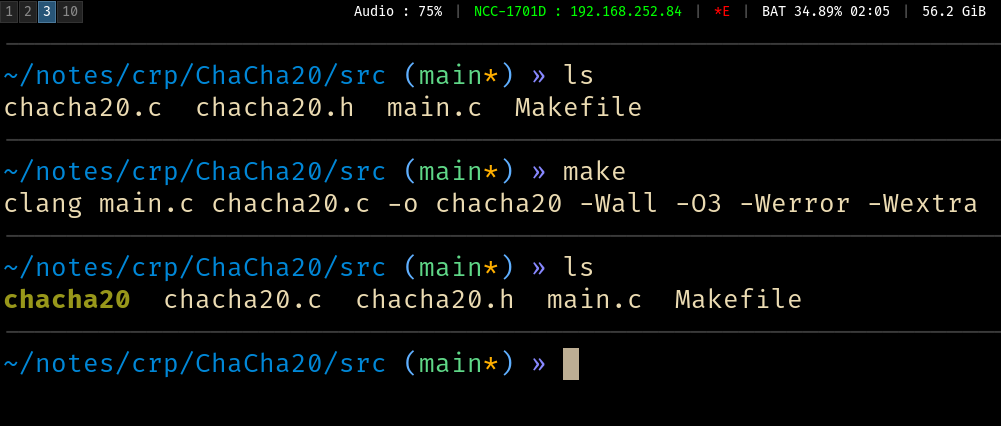
\includegraphics[width=0.9\textwidth]{../assets/1_make.png}
        \caption{Automated compilation using GNU Make}
	\label{image}
\end{figure}

A suitable Makefile has been used for speeding up recompilation time.

GNU Make is a build automation tool that reads Makefile instructions to compile code efficiently, tracking dependencies for minimal recompilation \cite{gnu_make}.
It uses rules of the form target: dependencies followed by commands to build the target.
It supports variables, conditionals, and functions for flexible build configurations.

The clang compiler has been utilized, with the address sanitizer in development, and with level 3 optimization in release mode. \cite{clang_manual}

AddressSanitizer (ASan) is a memory error detector for C/C++ programs, part of GCC and Clang. It detects out-of-bounds access, use-after-free, use-after-scope, and memory leaks.
ASan adds runtime checks, making programs slightly slower and more memory-intensive. It provides clear error messages with stack traces for quick debugging \cite{clang_address_sanitizer}.

-O3 in GCC is designed for performance-intensive applications where speed is a priority.
In addition to the optimizations at the -O2 level, -O3 includes optimizations like aggressive inlining, loop unrolling, and vectorization.

These optimizations can result in significant performance gains for programs that benefit from highly parallelized execution or intensive computational workloads.
However, -O3 can sometimes lead to larger binary sizes, as more functions may be inlined, and loops are unrolled to reduce loop control overhead. While this typically improves performance, the increased code size can potentially lead to cache misses and slower performance on certain systems, especially those with limited memory or cache.

\section{Encryption}
\begin{figure}[h]
	\centering
	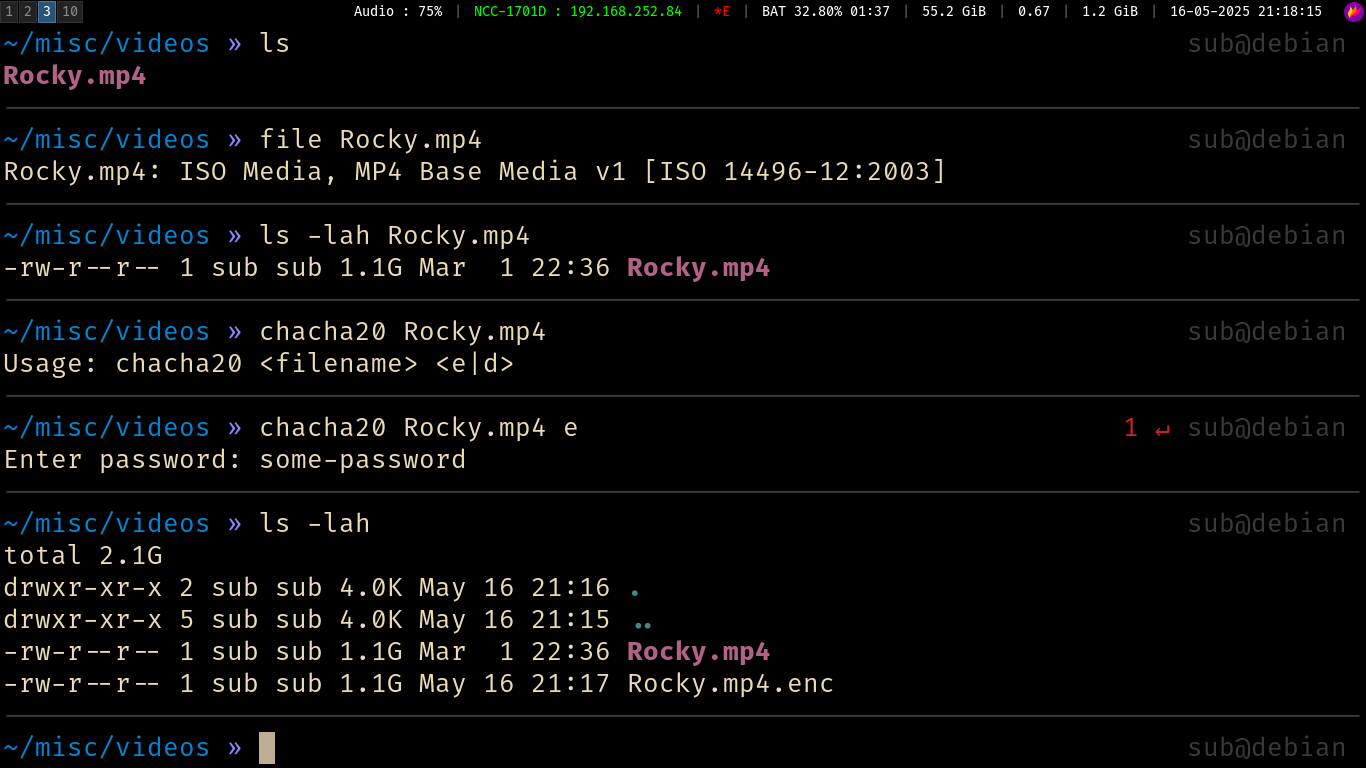
\includegraphics[width=0.9\textwidth]{../assets/2_encryption.png}
        \caption{Usage help message and encryption}
	\label{image}
\end{figure}

We demonstrate usage of the binary on a large file (1.1GiB).

This also demonstrates the capability of modern stream ciphers to act not only on ASCII text data, but data at the binary level encoded in a multitude of formats.

The program delivers an appropriate message when flags are not correctly provided.

\section{Decryption}
\begin{figure}[h]
	\centering
	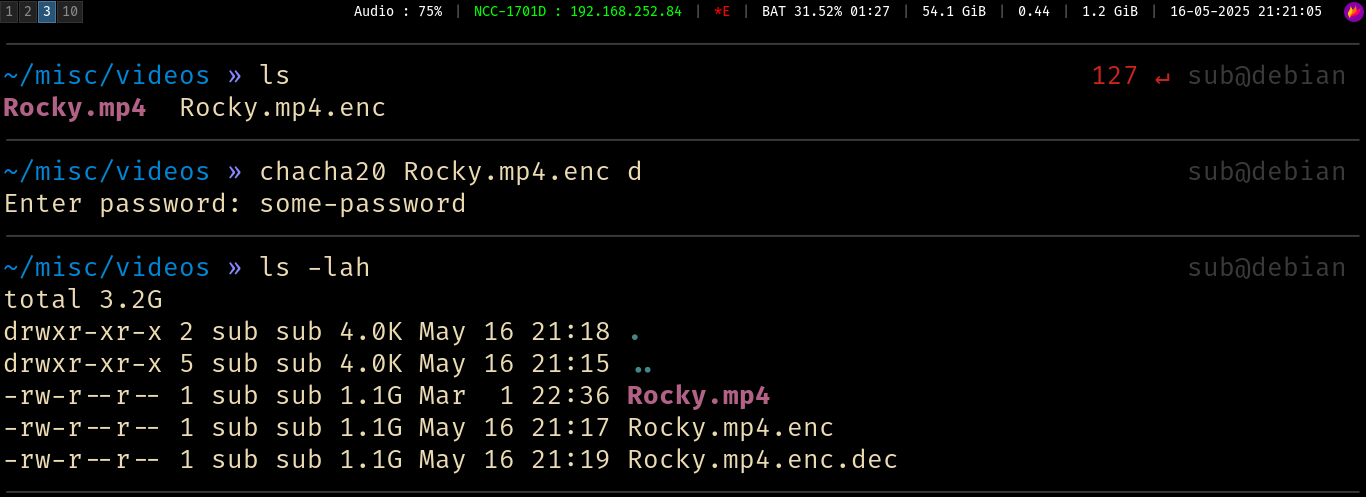
\includegraphics[width=0.9\textwidth]{../assets/3_decryption.png}
        \caption{Decryption with authenticity validation}
	\label{image}
\end{figure}

This process shows the symmetric-key nature of the algorithm, while also demonstrating the decryption process.

We note that the file size of the original file, encrypted file, and the decrypted file all remain the same.

This consistency in file size is a characteristic of stream ciphers like ChaCha20, where each byte of plaintext is directly transformed into a corresponding byte of ciphertext without altering the overall length.
The decrypted file is an exact byte-for-byte replica of the original, confirming the integrity of the encryption and decryption process.

\section{Validation}
\begin{figure}[H]
	\centering
	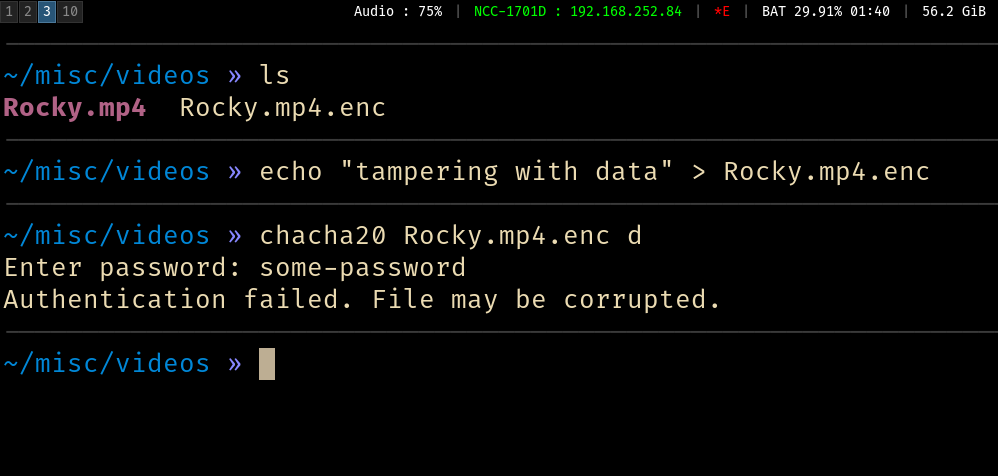
\includegraphics[width=0.9\textwidth]{../assets/4_Poly-1305.png}
        \caption{Invalid MAC signature detection and invalidation of data}
	\label{image}
\end{figure}

This test demonstrates the integrity protection provided by ChaCha20 with Poly1305 authentication mechanism.

By modifying even a single byte of the encrypted file, the decryption process fails with an authentication error.
This behavior ensures that any unauthorized modification of the ciphertext is immediately detected, protecting the integrity and authenticity of the data.



%   \begin{table}[h!]
%   \centering
%   \begin{tabular}{l l l l}
%   \toprule
%   Size & Column 2 & Column 3 & Column 4 \\ 
%   \midrule
%   1 MiB  & Row 1,2  & Row 1,3  & Row 1,4  \\ 
%   10 MiB & Row 2,2  & Row 2,3  & Row 2,4  \\ 
%   100 MiB  & Row 3,2  & Row 3,3  & Row 3,4  \\ 
%   \bottomrule
%   \end{tabular}
%   \caption{Benchmarking the program with an i5-2520M processor}
%   \end{table}


\chapter{Conclusion and Future Work}
%% Briefly summarize the important results and conclusions presented in the work.

In conclusion, this AAT examined the ChaCha20 stream cipher, focusing on its design, cryptographic security, and practical application when paired with Poly1305 for message authentication.
ChaCha20, designed as a secure, high-performance alternative to traditional stream ciphers like RC4 and block ciphers such as AES, exhibits a unique approach based on non-cryptanalytic techniques.
This methodology has proven to provide strong security guarantees, making ChaCha20 an effective solution for mitigating common attacks such as those targeting older ciphers.
Furthermore, the careful choice of rotation and quarter-round operations within ChaCha20 ensures that it remains resistant to differential and linear cryptanalysis, solidifying its trustworthiness in cryptographic systems.

The we also emphasized the significance of Poly1305 as a message authentication code (MAC), which, when combined with ChaCha20, enables authenticated encryption.
Poly1305's ability to provide both confidentiality and integrity through a single operation is crucial, as it mitigates the risk of potential man-in-the-middle attacks and guarantees that the integrity of transmitted data remains intact.
This combination of ChaCha20 with Poly1305 has garnered widespread adoption in protocols like TLS and is featured in popular systems such as Google's QUIC protocol, where both speed and security are paramount.

Performance evaluation results presented in this work further underscore the practical advantages of ChaCha20.
Unlike AES, which can be dependent on hardware acceleration for optimal performance, ChaCha20 is highly efficient in software implementations, making it particularly well-suited for environments with limited hardware support or resource constraints.

Ultimately, this work reinforces the credibility and utility of ChaCha20 as a highly secure and efficient cryptographic solution.
The combination of ChaCha20 and Poly1305 offers a versatile and reliable approach to authenticated encryption, making it an attractive alternative to established cryptographic schemes.
As cryptographic needs evolve, ChaCha20-Poly1305 remains a strong candidate for future developments in cryptographic systems, providing a balanced approach to both speed and security\cite{duck_ai}.

% Bibliography
\fontsize{12}{8}\selectfont
\bibliographystyle{unsrt}
\bibliography{main}

\end{document}
